\documentclass[11pt]{article}

\usepackage[margin=1in]{geometry}
\usepackage{amsmath,amssymb,amsthm}
\usepackage{enumitem}
\usepackage{tikz}
\usetikzlibrary{arrows.meta}

\setlength{\parindent}{0pt}
\setlist[enumerate]{itemsep=0.9em}

\tikzset{
  qarrow/.style={-{Stealth[length=5pt,width=4pt]}, line width=0.45pt}
}

\newcommand{\points}[1]{\textit{(#1 points)}}

\newcommand{\quiverDMain}{%
  \begin{tikzpicture}[baseline=(current bounding box.center), x=1cm, y=1cm]
    \node (v1) at (0,0) {$1$};
    \node (v2) at (1.8,0) {$2$};
    \node (v3) at (3.6,0) {$3$};
    \node (v4) at (5.0,0.9) {$4$};
    \node (v5) at (5.0,-0.9) {$5$};
    \draw[qarrow] (v1.east) -- (v2.west);
    \draw[qarrow] (v3.west) -- (v2.east);
    \draw[qarrow] (v3.north east) -- (v4.west);
    \draw[qarrow] (v3.south east) -- (v5.west);
  \end{tikzpicture}%
}

\newcommand{\quiverDTwo}{%
  \begin{tikzpicture}[baseline=(current bounding box.center), x=1cm, y=1cm]
    \node (v1) at (0,0) {$1$};
    \node (v2) at (1.8,0) {$2$};
    \node (v3) at (3.6,0) {$3$};
    \node (v4) at (5.0,0.9) {$4$};
    \node (v5) at (5.0,-0.9) {$5$};
    \draw[qarrow] (v2.west) -- (v1.east);
    \draw[qarrow] (v3.west) -- (v2.east);
    \draw[qarrow] (v3.north east) -- (v4.west);
    \draw[qarrow] (v5.west) -- (v3.south east);
  \end{tikzpicture}%
}

\newcommand{\quiverDThree}{%
  \begin{tikzpicture}[baseline=(current bounding box.center), x=1cm, y=1cm]
    \node (v1) at (0,0) {$1$};
    \node (v2) at (1.8,0) {$2$};
    \node (v3) at (3.6,0) {$3$};
    \node (v4) at (5.0,0.9) {$4$};
    \node (v5) at (5.0,-0.9) {$5$};
    \draw[qarrow] (v1.east) -- (v2.west);
    \draw[qarrow] (v2.east) -- (v3.west);
    \draw[qarrow] (v4.west) -- (v3.north east);
    \draw[qarrow] (v5.west) -- (v3.south east);
  \end{tikzpicture}%
}

\newcommand{\quiverDFour}{%
  \begin{tikzpicture}[baseline=(current bounding box.center), x=1cm, y=1cm]
    \node (v1) at (0,0) {$1$};
    \node (v2) at (1.8,0) {$2$};
    \node (v3) at (3.6,0) {$3$};
    \node (v4) at (5.0,0.9) {$4$};
    \node (v5) at (5.0,-0.9) {$5$};
    \draw[qarrow] (v2.west) -- (v1.east);
    \draw[qarrow] (v2.east) -- (v3.west);
    \draw[qarrow] (v3.north east) -- (v4.west);
    \draw[qarrow] (v5.west) -- (v3.south east);
  \end{tikzpicture}%
}

\newcommand{\quiverAFive}{%
  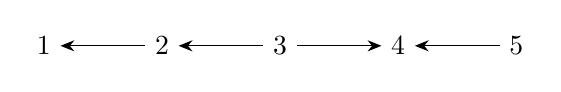
\begin{tikzpicture}[baseline=(current bounding box.center), x=1cm, y=1cm]
    \node (v1) at (0,0) {$1$};
    \node (v2) at (1.5,0) {$2$};
    \node (v3) at (3.0,0) {$3$};
    \node (v4) at (4.5,0) {$4$};
    \node (v5) at (6.0,0) {$5$};
    \draw[qarrow] (v2.west) -- (v1.east);
    \draw[qarrow] (v3.west) -- (v2.east);
    \draw[qarrow] (v3.east) -- (v4.west);
    \draw[qarrow] (v5.west) -- (v4.east);
  \end{tikzpicture}%
}

\newcommand{\quiverASix}{%
  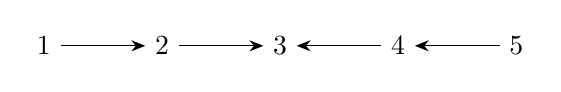
\begin{tikzpicture}[baseline=(current bounding box.center), x=1cm, y=1cm]
    \node (v1) at (0,0) {$1$};
    \node (v2) at (1.5,0) {$2$};
    \node (v3) at (3.0,0) {$3$};
    \node (v4) at (4.5,0) {$4$};
    \node (v5) at (6.0,0) {$5$};
    \draw[qarrow] (v1.east) -- (v2.west);
    \draw[qarrow] (v2.east) -- (v3.west);
    \draw[qarrow] (v4.west) -- (v3.east);
    \draw[qarrow] (v5.west) -- (v4.east);
  \end{tikzpicture}%
}

\newcommand{\quiverASeven}{%
  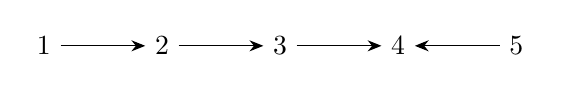
\begin{tikzpicture}[baseline=(current bounding box.center), x=1cm, y=1cm]
    \node (v1) at (0,0) {$1$};
    \node (v2) at (1.5,0) {$2$};
    \node (v3) at (3.0,0) {$3$};
    \node (v4) at (4.5,0) {$4$};
    \node (v5) at (6.0,0) {$5$};
    \draw[qarrow] (v1.east) -- (v2.west);
    \draw[qarrow] (v2.east) -- (v3.west);
    \draw[qarrow] (v3.east) -- (v4.west);
    \draw[qarrow] (v5.west) -- (v4.east);
  \end{tikzpicture}%
}

\begin{document}

\begin{center}
  {\Large\bfseries Final Exam - Applied Abstract Algebra}\\[0.4em]
  {\large\bfseries June 9th, 2026}
\end{center}

\section*{First Problem Variants}

\begin{enumerate}[label=\textbf{Variant \arabic*.}, leftmargin=*, itemsep=1.4em]
  \item % Source: final-applied-abstract-algebra-2026.pdf
    \points{40} Let $Q$ be a quiver:
    \[
      \quiverDMain
    \]
    \begin{enumerate}[label=\alph*)., leftmargin=2em, itemsep=0.3em]
      \item Construct $P(3)$ and $I(2)$ and using projective and injective resolution calculate
        $\tau(P(3))$ and $\tau^{-1}(I(2))$, where $\tau$ denotes the Auslander-Reiten translation.
      \item Construct a triangulation of punctured polygon corresponding to $Q$ and find which
        arcs with respect to this triangulation correspond to $P(3)$, $I(2)$, $\tau(P(3))$,
        $\tau^{-1}(I(2))$ and to indecomposable representation of dimension vector
        $(1,2,2,1,1)$.
    \end{enumerate}
    \begin{proof}
      The projective $P(i)$ is spanned by paths starting at $i$, and the injective
      $I(i)$ is spanned by paths ending at $i$. Hence
      \[
        \dim P(3)=(0,1,1,1,1),\qquad
        \dim I(2)=(1,1,1,0,0).
      \]
      The nonzero maps in $P(3)$ are the identity maps on the arrows
      $3\to2$, $3\to4$, and $3\to5$; the nonzero maps in $I(2)$ are the
      identity maps on $1\to2$ and $3\to2$.

      Since $P(3)$ is projective, its minimal projective resolution is
      $0\to0\to P(3)\to P(3)\to0$, so applying the Nakayama definition of
      Auslander-Reiten translation gives $\tau P(3)=0$. Similarly, $I(2)$ is
      injective, so $\tau^{-1}I(2)=0$.

      Let $T_Q=\{\gamma_1,\ldots,\gamma_5\}$ be the triangulation of the
      punctured pentagon obtained from $Q$ by Schiffler's construction, with
      $\gamma_i$ corresponding to the vertex $i$. Let $R$ denote elementary
      clockwise rotation, with tag change at the puncture. Then
      \[
        P(3)\leftrightarrow R^{-1}\gamma_3,\qquad
        I(2)\leftrightarrow R\gamma_2.
      \]
      The actual objects $\tau P(3)$ and $\tau^{-1}I(2)$ are zero in
      $\operatorname{rep}Q$; formally rotating the arcs gives the boundary
      triangulation arcs $\gamma_3$ and $\gamma_2$, respectively.

      The indecomposable representation of dimension vector $(1,2,2,1,1)$ may be
      written as
      \[
        X_1=X_4=X_5=k,\qquad X_2=X_3=k^2,
      \]
      with arrow maps
      \[
        X_{1\to2}=\binom{1}{1},\qquad
        X_{3\to2}=I_2,\qquad
        X_{3\to4}=(1\ 0),\qquad
        X_{3\to5}=(0\ 1).
      \]
      If $f$ is an endomorphism of $X$, then the two maps out of $X_3$ force
      $f_3$ to be diagonal, the identity map $X_3\to X_2$ gives $f_2=f_3$, and
      the map $X_1\to X_2$ forces the two diagonal entries to be equal. Thus
      $\operatorname{End}(X)=k$, so $X$ is indecomposable. Geometrically, $X$
      corresponds to the unique arc $\rho$ not in $T_Q$ such that
      \[
        (e(\rho,\gamma_1),\ldots,e(\rho,\gamma_5))=(1,2,2,1,1).
      \]
    \end{proof}

  \item % Source: final-applied-abstract-algebra-2026-2.pdf
    \points{40} Let $Q$ be a quiver:
    \[
      \quiverDTwo
    \]
    \begin{enumerate}[label=\alph*)., leftmargin=2em, itemsep=0.3em]
      \item Construct $P(3)$ and $I(2)$ and using projective and injective resolution calculate
        $\tau(P(3))$ and $\tau^{-1}(I(2))$, where $\tau$ denotes the Auslander-Reiten translation.
      \item Construct a triangulation of punctured polygon corresponding to $Q$ and find which
        arcs with respect to this triangulation correspond to $P(3)$, $I(2)$, $\tau(P(3))$,
        $\tau^{-1}(I(2))$ and to indecomposable representation of dimension vector
        $(1,2,2,1,1)$.
    \end{enumerate}
    \begin{proof}
      By the path description of projectives and injectives,
      \[
        \dim P(3)=(1,1,1,1,0),\qquad
        \dim I(2)=(0,1,1,0,1).
      \]
      The nonzero maps in $P(3)$ are identities along $3\to2$, $2\to1$, and
      $3\to4$; the nonzero maps in $I(2)$ are identities along $5\to3$ and
      $3\to2$. Since $P(3)$ is projective and $I(2)$ is injective,
      \[
        \tau P(3)=0,\qquad \tau^{-1}I(2)=0.
      \]

      Construct the punctured-pentagon triangulation
      $T_Q=\{\gamma_1,\ldots,\gamma_5\}$ by Schiffler's rule, labeling
      $\gamma_i$ by the vertex $i$. With $R$ the clockwise tagged rotation,
      \[
        P(3)\leftrightarrow R^{-1}\gamma_3,\qquad
        I(2)\leftrightarrow R\gamma_2.
      \]
      Thus the formal rotated arcs for $\tau P(3)$ and $\tau^{-1}I(2)$ are
      $\gamma_3$ and $\gamma_2$, while the actual representations are zero.

      For the dimension vector $(1,2,2,1,1)$ take
      $X_1=X_4=X_5=k$ and $X_2=X_3=k^2$, with maps
      \[
        X_{2\to1}=(1\ -1),\qquad
        X_{3\to2}=I_2,\qquad
        X_{3\to4}=(1\ 0),\qquad
        X_{5\to3}=\binom{1}{0}.
      \]
      The endomorphism relations force the common matrix on $X_2$ and $X_3$ to be
      diagonal, and then the maps to $X_1$ and $X_4$ force the two diagonal entries
      to agree. Hence $\operatorname{End}(X)=k$, so $X$ is indecomposable. It is
      the arc $\rho$ with crossing vector
      \[
        (e(\rho,\gamma_1),\ldots,e(\rho,\gamma_5))=(1,2,2,1,1).
      \]
    \end{proof}

  \item % Source: final-applied-abstract-algebra-2026-3.pdf
    \points{40} Let $Q$ be a quiver:
    \[
      \quiverDThree
    \]
    \begin{enumerate}[label=\alph*)., leftmargin=2em, itemsep=0.3em]
      \item Construct $P(2)$ and $I(3)$ and using projective and injective resolution calculate
        $\tau(P(2))$ and $\tau^{-1}(I(3))$, where $\tau$ denotes the Auslander-Reiten translation.
      \item Construct a triangulation of punctured polygon corresponding to $Q$ and find which
        arcs with respect to this triangulation correspond to $P(2)$, $I(3)$, $\tau(P(2))$,
        $\tau^{-1}(I(3))$ and to indecomposable representation of dimension vector
        $(1,2,2,1,1)$.
    \end{enumerate}
    \begin{proof}
      The projective and injective representations are
      \[
        \dim P(2)=(0,1,1,0,0),\qquad
        \dim I(3)=(1,1,1,1,1).
      \]
      In $P(2)$ the only nonzero arrow map is the identity on $2\to3$; in $I(3)$
      all four arrow maps are identities. Since $P(2)$ is projective and $I(3)$ is
      injective,
      \[
        \tau P(2)=0,\qquad \tau^{-1}I(3)=0.
      \]

      Let $T_Q=\{\gamma_1,\ldots,\gamma_5\}$ be the punctured-pentagon
      triangulation associated to this orientation. Then
      \[
        P(2)\leftrightarrow R^{-1}\gamma_2,\qquad
        I(3)\leftrightarrow R\gamma_3.
      \]
      The formal arcs obtained by rotating once are $\gamma_2$ and $\gamma_3$;
      these are triangulation arcs, while the corresponding translated
      representations in $\operatorname{rep}Q$ are zero.

      The required indecomposable of dimension vector $(1,2,2,1,1)$ is obtained by
      taking $X_1=X_4=X_5=k$, $X_2=X_3=k^2$, and
      \[
        X_{1\to2}=\binom{1}{1},\qquad
        X_{2\to3}=I_2,\qquad
        X_{4\to3}=\binom{0}{1},\qquad
        X_{5\to3}=\binom{1}{0}.
      \]
      The two maps into $X_3$ make the common endomorphism of $X_2$ and $X_3$
      diagonal in the standard basis, and the map from $X_1$ forces the two
      diagonal entries to be equal. Therefore $\operatorname{End}(X)=k$, so $X$ is
      indecomposable. It corresponds to the unique arc $\rho$ with crossing vector
      $(1,2,2,1,1)$ against the arcs $\gamma_i$.
    \end{proof}

  \item % Source: final-applied-abstract-algebra-2026-4.pdf
    \points{40} Let $Q$ be a quiver:
    \[
      \quiverDFour
    \]
    \begin{enumerate}[label=\alph*)., leftmargin=2em, itemsep=0.3em]
      \item Construct $P(2)$ and $I(3)$ and using projective and injective resolution calculate
        $\tau(P(2))$ and $\tau^{-1}(I(3))$, where $\tau$ denotes the Auslander-Reiten translation.
      \item Construct a triangulation of punctured polygon corresponding to $Q$ and find which
        arcs with respect to this triangulation correspond to $P(2)$, $I(3)$, $\tau(P(2))$,
        $\tau^{-1}(I(3))$ and to indecomposable representation of dimension vector
        $(1,2,2,1,1)$.
    \end{enumerate}
    \begin{proof}
      The path descriptions give
      \[
        \dim P(2)=(1,1,1,1,0),\qquad
        \dim I(3)=(0,1,1,0,1).
      \]
      The nonzero maps in $P(2)$ are identities along $2\to1$, $2\to3$, and
      $3\to4$; the nonzero maps in $I(3)$ are identities along $2\to3$ and
      $5\to3$. Hence
      \[
        \tau P(2)=0,\qquad \tau^{-1}I(3)=0.
      \]

      If $T_Q=\{\gamma_1,\ldots,\gamma_5\}$ is the corresponding triangulation of
      the punctured pentagon and $R$ is clockwise tagged rotation, then
      \[
        P(2)\leftrightarrow R^{-1}\gamma_2,\qquad
        I(3)\leftrightarrow R\gamma_3.
      \]
      Thus the formal arcs for the two translated terms are $\gamma_2$ and
      $\gamma_3$, although the actual representations are zero.

      For the vector $(1,2,2,1,1)$ take $X_1=X_4=X_5=k$ and $X_2=X_3=k^2$ with
      \[
        X_{2\to1}=(1\ -1),\qquad
        X_{2\to3}=I_2,\qquad
        X_{3\to4}=(1\ 0),\qquad
        X_{5\to3}=\binom{1}{0}.
      \]
      The same endomorphism calculation as above gives
      $\operatorname{End}(X)=k$, so $X$ is indecomposable. In the punctured
      pentagon it is the unique arc $\rho$ satisfying
      \[
        (e(\rho,\gamma_1),\ldots,e(\rho,\gamma_5))=(1,2,2,1,1).
      \]
    \end{proof}

  \item % Source: final-applied-abstract-algebra-2026-5.pdf
    \points{40} Let $Q$ be a quiver:
    \[
      \quiverAFive
    \]
    \begin{enumerate}[label=\alph*)., leftmargin=2em, itemsep=0.3em]
      \item Compute the Auslander-Reiten quiver for $Q$. Calculate $\operatorname{Hom}(P(3),I(4))$.
      \item Construct a triangulation of polygon corresponding to $Q$ and find which arcs with
        respect to this triangulation correspond to $P(3)$, $I(4)$, $\tau(P(3))$,
        $\tau^{-1}(I(4))$ and to indecomposable representation of dimension vector
        $(1,1,1,1,1)$.
    \end{enumerate}
    \begin{proof}
      Write $X_{ab}$ for the interval representation supported on
      $a,a+1,\ldots,b$. The vertices of the Auslander-Reiten quiver are all
      $X_{ab}$ with $1\le a\le b\le5$, and its irreducible arrows are
      \[
      \begin{gathered}
        X_{11}\to X_{12},\quad
        X_{12}\to X_{14},X_{22},\quad
        X_{13}\to X_{23},\\
        X_{14}\to X_{15},X_{24},\quad
        X_{15}\to X_{13},X_{25},\quad
        X_{22}\to X_{24},\\
        X_{23}\to X_{33},\quad
        X_{24}\to X_{25},X_{34},\quad
        X_{25}\to X_{23},X_{35},\\
        X_{34}\to X_{35},\quad
        X_{35}\to X_{33},X_{55},\quad
        X_{44}\to X_{14},X_{45},\quad
        X_{45}\to X_{15}.
      \end{gathered}
      \]
      Here $P(3)=X_{14}$ and $I(4)=X_{35}$. Since
      $\operatorname{Hom}(P(i),M)\cong M_i$ naturally,
      \[
        \operatorname{Hom}(P(3),I(4))\cong I(4)_3\cong k,
      \]
      so $\dim\operatorname{Hom}(P(3),I(4))=1$.

      Number the vertices of an $8$-gon clockwise. A triangulation corresponding
      to $Q$ is
      \[
        T_1=(1,3),\quad T_2=(3,8),\quad T_3=(3,7),\quad
        T_4=(4,7),\quad T_5=(4,6).
      \]
      A diagonal not in the triangulation represents the interval whose support is
      exactly the set of triangulation diagonals that it crosses. Thus
      \[
        P(3)=X_{14}\leftrightarrow(2,6),\qquad
        I(4)=X_{35}\leftrightarrow(5,8),\qquad
        X_{15}\leftrightarrow(2,5).
      \]
      In $\operatorname{rep}Q$, $\tau P(3)=0$ and $\tau^{-1}I(4)=0$. Under the
      formal polygon rotation, these boundary positions are the triangulation
      diagonals $T_3=(3,7)$ and $T_4=(4,7)$, respectively.
    \end{proof}

  \item % Source: final-applied-abstract-algebra-2026-6.pdf
    \points{40} Let $Q$ be a quiver:
    \[
      \quiverASix
    \]
    \begin{enumerate}[label=\alph*)., leftmargin=2em, itemsep=0.3em]
      \item Compute the Auslander-Reiten quiver for $Q$. Calculate $\operatorname{Hom}(P(1),I(3))$.
      \item Construct a triangulation of polygon corresponding to $Q$ and find which arcs with
        respect to this triangulation correspond to $P(1)$, $I(3)$, $\tau(P(1))$,
        $\tau^{-1}(I(3))$ and to indecomposable representation of dimension vector
        $(1,1,1,1,1)$.
    \end{enumerate}
    \begin{proof}
      Again let $X_{ab}$ denote the interval representation supported on
      $a,\ldots,b$. The Auslander-Reiten quiver has vertices $X_{ab}$,
      $1\le a\le b\le5$, and irreducible arrows
      \[
      \begin{gathered}
        X_{12}\to X_{11},\quad
        X_{13}\to X_{14},\quad
        X_{14}\to X_{15},X_{44},\quad
        X_{15}\to X_{12},X_{45},\\
        X_{22}\to X_{12},\quad
        X_{23}\to X_{13},X_{24},\quad
        X_{24}\to X_{14},X_{25},\\
        X_{25}\to X_{15},X_{22},\quad
        X_{33}\to X_{23},X_{34},\\
        X_{34}\to X_{24},X_{35},\quad
        X_{35}\to X_{25},\quad
        X_{44}\to X_{45},\quad
        X_{45}\to X_{55}.
      \end{gathered}
      \]
      We have $P(1)=X_{13}$ and $I(3)=X_{15}$. Therefore
      \[
        \operatorname{Hom}(P(1),I(3))\cong I(3)_1\cong k,
      \]
      and the Hom space has dimension $1$.

      A corresponding triangulation of the clockwise numbered $8$-gon is
      \[
        T_1=(1,3),\quad T_2=(1,4),\quad T_3=(1,5),\quad
        T_4=(5,8),\quad T_5=(5,7).
      \]
      The relevant diagonals are
      \[
        P(1)=X_{13}\leftrightarrow(2,8),\qquad
        I(3)=X_{15}\leftrightarrow(2,6),\qquad
        X_{15}\leftrightarrow(2,6).
      \]
      The actual translated representations are
      $\tau P(1)=0$ and $\tau^{-1}I(3)=0$; the formal rotated arcs are
      $T_1=(1,3)$ and $T_3=(1,5)$.
    \end{proof}

  \item % Source: final-applied-abstract-algebra-2026-7.pdf
    \points{40} Let $Q$ be a quiver:
    \[
      \quiverASeven
    \]
    \begin{enumerate}[label=\alph*)., leftmargin=2em, itemsep=0.3em]
      \item Compute the Auslander-Reiten quiver for $Q$. Calculate $\operatorname{Hom}(P(1),I(4))$.
      \item Construct a triangulation of polygon corresponding to $Q$ and find which arcs with
        respect to this triangulation correspond to $P(1)$, $I(4)$, $\tau(P(1))$,
        $\tau^{-1}(I(4))$ and to indecomposable representation of dimension vector
        $(1,1,1,1,1)$.
    \end{enumerate}
    \begin{proof}
      Let $X_{ab}$ be the interval representation supported on $a,\ldots,b$. The
      Auslander-Reiten quiver has irreducible arrows
      \[
      \begin{gathered}
        X_{12}\to X_{11},\quad
        X_{13}\to X_{12},\quad
        X_{14}\to X_{15},\quad
        X_{15}\to X_{13},X_{55},\\
        X_{22}\to X_{12},\quad
        X_{23}\to X_{13},X_{22},\quad
        X_{24}\to X_{14},X_{25},\\
        X_{25}\to X_{15},X_{23},\quad
        X_{33}\to X_{23},\quad
        X_{34}\to X_{24},X_{35},\\
        X_{35}\to X_{25},X_{33},\quad
        X_{44}\to X_{34},X_{45},\quad
        X_{45}\to X_{35}.
      \end{gathered}
      \]
      Here $P(1)=X_{14}$ and $I(4)=X_{15}$, so
      \[
        \operatorname{Hom}(P(1),I(4))\cong I(4)_1\cong k.
      \]
      Thus $\dim\operatorname{Hom}(P(1),I(4))=1$.

      One triangulation of the clockwise numbered $8$-gon corresponding to this
      orientation is
      \[
        T_1=(1,3),\quad T_2=(1,4),\quad T_3=(1,5),\quad
        T_4=(1,6),\quad T_5=(6,8).
      \]
      The relevant diagonals are
      \[
        P(1)=X_{14}\leftrightarrow(2,8),\qquad
        I(4)=X_{15}\leftrightarrow(2,7),\qquad
        X_{15}\leftrightarrow(2,7).
      \]
      The actual translated representations are zero:
      $\tau P(1)=0$ and $\tau^{-1}I(4)=0$. The formal polygon rotations land on
      the triangulation diagonals $T_1=(1,3)$ and $T_4=(1,6)$.
    \end{proof}
\end{enumerate}

\section*{Common Problems}

\textit{Choose up to three problems from this list to submit.}

\begin{enumerate}[label=\arabic*., leftmargin=2em, itemsep=1.1em]
  \item \points{20} Prove that $P$ is projective if and only if
    $\operatorname{Ext}^1(P,N)=0$ for all representations $N$.
    \begin{proof}
      If $P$ is projective, every short exact sequence
      \[
        0\to N\to E\to P\to0
      \]
      splits, since the identity map of $P$ lifts through $E\twoheadrightarrow P$.
      Hence every extension of $P$ by $N$ is trivial, so
      $\operatorname{Ext}^1(P,N)=0$.

      Conversely, assume that $\operatorname{Ext}^1(P,N)=0$ for every $N$. Let
      $g:M\twoheadrightarrow X$ be an epimorphism and let $f:P\to X$ be a map.
      Form the pullback
      \[
        E=M\times_X P=\{(m,p)\mid g(m)=f(p)\}.
      \]
      Then
      \[
        0\to \ker g\to E\to P\to0
      \]
      is exact. Its class lies in $\operatorname{Ext}^1(P,\ker g)=0$, so it
      splits. A section $P\to E$, followed by the projection $E\to M$, gives a
      lift of $f$ through $g$. Thus $\operatorname{Hom}(P,-)$ sends epimorphisms
      to epimorphisms, and $P$ is projective.
    \end{proof}

  \item \points{20} Let $M \in \operatorname{rep} Q$ and
    \[
      0 \to P_1 \to P_0 \to M \to 0
    \]
    be standard projective resolution. Show that
    \[
      0 \to D(M) \to D(P_0) \to D(P_1) \to 0
    \]
    is the injective resolution for $D(M) \in \operatorname{rep} Q^{\mathrm{op}}$.
    Show that duality functor $D$ takes a minimal projective resolution for $M$ to
    a injective envelope for $D(M)$.
    \begin{proof}
      Write $D=\operatorname{Hom}_k(-,k)$. Since all vector spaces are
      finite-dimensional, $D$ is exact and contravariant. Applying $D$ to
      \[
        0\to P_1\to P_0\to M\to0
      \]
      gives an exact sequence
      \[
        0\to D(M)\to D(P_0)\to D(P_1)\to0.
      \]
      For every vertex $i$, the dual of the projective $P_Q(i)$ is the injective
      $I_{Q^{\mathrm{op}}}(i)$: a path $i\to j$ in $Q$ is the same as a path
      $j\to i$ in $Q^{\mathrm{op}}$ after reversing arrows and dualizing. Hence
      $D(P_0)$ and $D(P_1)$ are injective representations of $Q^{\mathrm{op}}$.
      Therefore the displayed sequence is an injective resolution of $D(M)$.

      If the projective resolution is minimal, then the map $P_0\twoheadrightarrow
      M$ is a projective cover. Its dual $D(M)\hookrightarrow D(P_0)$ is an
      essential monomorphism into an injective object: equivalently, if
      $a:D(P_0)\to D(P_0)$ satisfies $a|_{D(M)}=\operatorname{id}_{D(M)}$, then
      dualizing gives an endomorphism of $P_0$ over $M$, hence an automorphism by
      minimality of the projective cover. Thus $D(M)\hookrightarrow D(P_0)$ is an
      injective envelope, and the dual complex is the minimal injective resolution.
    \end{proof}

  \item \points{20} Let $g:M \to N$ be a surjective morphism between representations of
    $Q$, and let $P(i)$ be the projective representation at vertex $i$. Show that the map
    \[
      g_*:\operatorname{Hom}(P(i),M) \to \operatorname{Hom}(P(i),N)
    \]
    is surjective.
    \begin{proof}
      For every representation $X$ there is a natural isomorphism
      \[
        \operatorname{Hom}(P(i),X)\cong X_i,\qquad
        f\mapsto f_i(e_i),
      \]
      where $e_i$ is the trivial path at $i$. Under this identification, the map
      $g_*$ is exactly the component map $g_i:M_i\to N_i$. Since $g$ is
      surjective, each component $g_i$ is surjective. Hence $g_*$ is surjective.
    \end{proof}

  \item \points{20} Show that for any $Q$ the representations $I(i)$, $i \in Q_0$ are
    indecomposable.
    \begin{proof}
      In the finite acyclic setting, the dual Yoneda isomorphism gives
      \[
        \operatorname{Hom}(X,I(i))\cong D(X_i)
      \]
      naturally in $X$. Taking $X=I(i)$ yields
      \[
        \operatorname{End}(I(i))\cong D(I(i)_i).
      \]
      Since the only path from $i$ to $i$ is the trivial path, $I(i)_i\cong k$, and
      therefore $\operatorname{End}(I(i))\cong k$. If $I(i)=A\oplus B$ with both
      $A$ and $B$ nonzero, projection onto one summand would give a nonzero
      idempotent different from $1$ in $\operatorname{End}(I(i))$, impossible in
      the field $k$. Thus $I(i)$ is indecomposable.
    \end{proof}

  \item \points{20} Show that the smallest wild tree with valence at most $3$ at each
    vertex has $7$ vertices.
    \begin{proof}
      For acyclic quivers, representation type depends only on the underlying graph:
      Dynkin trees are finite type, Euclidean trees are tame, and all other connected
      trees are wild.

      No tree with at most five vertices is wild: a path is of type $A_n$, and under
      the maximum-valence-$3$ condition the only branched possibilities are $D_4$
      and $D_5$. With six vertices and maximum valence at most $3$, the possible
      trees are
      \[
        A_6,\qquad D_6,\qquad E_6,\qquad \widetilde D_5,
      \]
      which are Dynkin or Euclidean. Hence no such tree with at most six vertices
      is wild.

      Now consider the seven-vertex tree with edges
      \[
        ua,\quad ub,\quad uv,\quad vc,\quad vw,\quad wd.
      \]
      It has maximum valence $3$: the vertices $u$ and $v$ have valence $3$, the
      vertex $w$ has valence $2$, and $a,b,c,d$ are leaves. It is not Dynkin of
      type $A,D,E$, and it is not Euclidean: it is not a cycle, not one of the
      exceptional $\widetilde E$ diagrams, and it is not a $\widetilde D_n$ diagram
      because the two trivalent vertices are adjacent while one outer arm has length
      $2$. Therefore it is wild. Thus the smallest possible number of vertices is
      $7$.
    \end{proof}
\end{enumerate}

\end{document}
